
\documentclass[paper=a4, fontsize=11pt]{scrartcl} % A4 paper and 11pt font size

\usepackage[T1]{fontenc} % Use 8-bit encoding that has 256 glyphs
\usepackage{fourier} % Use the Adobe Utopia font for the document - comment this line to return to the LaTeX default
\usepackage[english]{babel} % English language/hyphenation
\usepackage{amsmath,amsfonts,amsthm} % Math packages
\usepackage{graphicx}
\usepackage{subfig}
\usepackage{caption}
\usepackage[section]{placeins}
\usepackage{sectsty} % Allows customizing section commands
\allsectionsfont{\centering \normalfont\scshape} % Make all sections centered, the default font and small caps
\numberwithin{equation}{section} % Number equations within sections (i.e. 1.1, 1.2, 2.1, 2.2 instead of 1, 2, 3, 4)
\numberwithin{figure}{section} % Number figures within sections (i.e. 1.1, 1.2, 2.1, 2.2 instead of 1, 2, 3, 4)
\numberwithin{table}{section} % Number tables within sections (i.e. 1.1, 1.2, 2.1, 2.2 instead of 1, 2, 3, 4)

\setlength\parindent{0pt} % Removes all indentation from paragraphs - comment this line for an assignment with lots of text

%----------------------------------------------------------------------------------------
%	TITLE SECTION
%----------------------------------------------------------------------------------------

\newcommand{\horrule}[1]{\rule{\linewidth}{#1}} % Create horizontal rule command with 1 argument of height

\title{	
\normalfont \normalsize 
\textsc{PH 481 Lab} \\ [25pt] % Your university, school and/or department name(s)
\horrule{2pt} \\[0.5cm] % Thin top horizontal rule
\huge Optics Lab 4\\ % The assignment title
\horrule{2pt} \\[0.5cm] % Thick bottom horizontal rule
}

\author{Harsukh Singh} % Your name

\date{\normalsize \today} % Today's date or a custom date

\begin{document}

\maketitle % Print the title
\section{Overview of Experiment}
This lab involved the study and use of the Fabry Perot Interferometer, the diagram of the interferometer is shown below.  The Interferometer are usually used to study interference patterns of waves. Interferometers can usually be divided into two separate parts, the amplitude splitting and wave front splitting. The Fabry Perot Interometer is a amplitude splitting interfometer, which makes use of the multiple reflections between two closely spaced glass plates. This results in multiple beams which can interfere with each other and when these beams are focused onto a surface they produce cocentric circle interference patters and  these ``new'' diffuse have lower amplitudes compared to the original wave, so in a sense the amplitude has been split. If  these new waves were brought together again it would create an interference pattern. 
\begin{figure}[htb]
\centering
\parbox{5cm}{
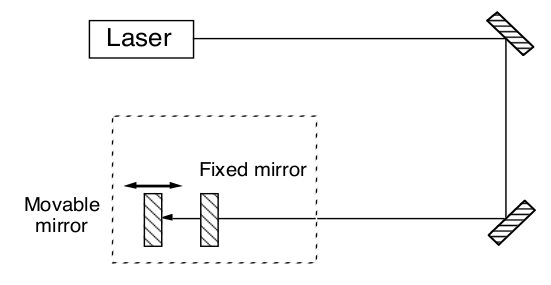
\includegraphics[width=5cm]{exp}
\caption{Experimental Set-up}
\label{fig:2figsA}}
\qquad
\begin{minipage}{5cm}
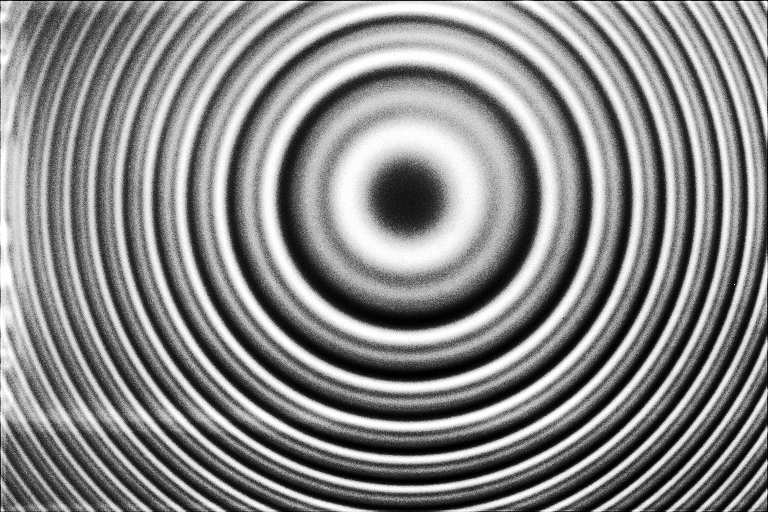
\includegraphics[width=5cm]{fpat}
\caption{Fabry Perot Pattern}
\label{fig:2figsB}
\end{minipage}
\end{figure}

The Fabry Perot obeys the same equation for the optical path difference is given by $ OPD = 2dcos(\theta)$. The Fabry Perot fringe pattern is described by a airy-disc equation, given below.
\begin{equation}
2dcos(\theta_m) = m\lambda_0 
\end{equation}
\begin{equation}
I(\delta) = \frac{I_0}{I+(\frac{2F}{\pi})^2 sin^2(\frac{\delta}{2})}
\end{equation}
Here F is the Finesse and $\delta$ is given by $\delta = 2kdcos(\theta)$. In this lab we tried measuring both the sodium and mercury doublet. The doublet is when the the drigense from two different wavelengths overlap at the center $(\theta = 0)$ so then, $2d = N_1\lambda_1 = N_2 \lambda_2$. The spacing between the mirrors is then changed until the fringes are resolved i.e. you can see two different fringe patterns. The equation for finesse we can derive from this is,
\begin{equation}
F = \frac{1}{\epsilon} = 2\frac{ d^{'''} -d^{'}}{d^{''} -d^{'}}
\end{equation}
 \section{Mercury Doublet}
 To set up the lab we aligned the laser to both mirrors on both glass plates of the interferometer so that the beams that meet the target are coinciding. This insures that beam is non-dispersive throughout the experiment and the interference pattern is observed. The translational stage is connected to a microcontroller for changing the displacement of the glass plate.  The fringe pattern is viewed by a camera connected to a computer that displays the fringe patten. Unfortunately we were unable to focus onto the fringes but we did use another lab groups data for analysis.
\begin{equation}
  \begin{tabular}{|l |r| }
    \hline
     d(m) & 0.0065561             \\ \hline
    d^{'} (m) & 0.0064660        \\ \hline
    d^{''}(m) & 0.006345             \\  \hline
    d^{'''}(m)& 0.0061452               \\  \hline
  \end{tabular}
\end{equation}
The calculated finesse is 5.34. And now we can plot the intensity of the Fabry-Perot Fringes. These are shown below
\begin{figure}[htb]
	\caption{Fabry-Perot fringes (I vs delta)}
		\begin{center}
			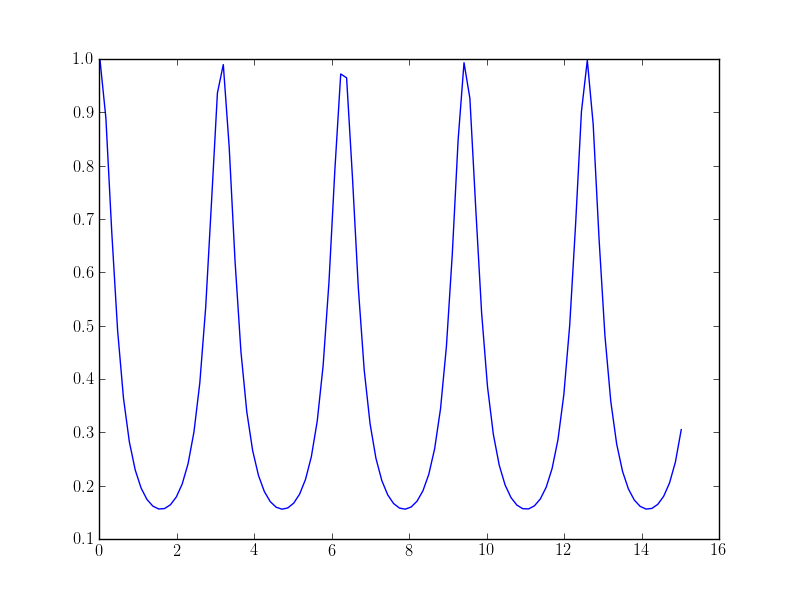
\includegraphics[scale=0.5]{fringes}
		\end{center}
\end{figure}
\section{Sodium Doublet}
In this part of the lab, we replaced the mercury lamp with a sodium lamp and we viewed the interference pattern but were unable to adjust the intensity of the interference pattern, to measure anything credible. The method of analysis is the same but for some odd reason, our experimental setup for this part did not produce any results. 
\section{Conclusion}
While we were unable to do some of this lab since we ran into some technical diffculties, we did go through the motions and tried getting reasonable results. 
%\begin{figure}[htb]
%\centering
%\parbox{5cm}{
%\includegraphics[width=5cm]{figure_1}
%\caption{ Reflection Coefficients}}
%\qquad
%\begin{minipage}{5cm}
%\includegraphics[width=5cm]{figure_2}
%\caption{Transmission Coefficients}
%\end{minipage}
%\end{figure}
%
%\begin{figure}[htb]
%\centering
%\parbox{5cm}{
%\includegraphics[width=5cm]{Epar}
%\caption{Electric Field Parallel to Incident Plane}
%\label{fig:2figsA}}
%\qquad
%\begin{minipage}{5cm}
%\includegraphics[width=5cm]{Eperp}
%\caption{Electric Field Perpendicular to Indicent Plane}
%\label{fig:2figsB}
%\end{minipage}
%%\end{figure}
%
%\section{Experiment 1.1:  Transmittance through Glass}
%\begin{figure}[!ht]
%	\caption{Experimental Set-Up}
%		\begin{center}
%			\includegraphics[scale=0.5]{transmittance}
%		\end{center}
%\end{figure}

%\begin{figure}[!ht]
%	\caption{Experimental Comparison to Theoretical Transmission Coefficients}
%		\begin{center}
%			\includegraphics[scale=0.5]{figure_3}
%		\end{center}
%\end{figure}
%
%\section{Experiment 1.2:  Reflectance from Frosted Glass}
%\begin{figure}[!ht]
%		\begin{center}
%			\includegraphics[scale=0.5]{reflectance}
%		\end{center}
%\caption{Reflectance from Frosted Glass}
%\end{figure}

%\section{Experiment 1.3: Refraction through glass slab}
%\begin{figure}[!ht]
%		\begin{center}
%			\includegraphics[scale=0.5]{GlassLab}
%		\end{center}
%\caption{Measuring the index of refraction through Glass Slab}
%\end{figure}g
% \begin{equation}
%sin(\theta_i -\theta_t) = \frac{l}{\frac{t}{cos(\theta_t)}}
% \end{equation}
% and,
% \begin{equation}
%n_{slab}  = \frac{n_1sin(\theta_1)}{sin(\theta_1-sin^{-1}(\frac{t}{\frac{l}{sin(\theta_i -\theta_t)}}))}
% \end{equation}
% Solving this $n_{slab} = 1.42$  and since most glass has a refractive index of ~1.5 this was pretty close.
 \end{document}
